\documentclass[a4paper,11pt,exos]{nsi} % COMPILE WITH DRAFT
\usepackage{pifont}
\usepackage{fontawesome5}

\begin{document}
\classe{\premiere spé}
\titre{Exercices - Premier degré}
\maketitle

\subsection*{Premier degré}
\exo{}
\begin{enumerate}
    \item 	Résoudre les équations suivantes :			\setlength{\columnseprule}{0pt}
    \begin{multicols}{4}
        \begin{enumerate}[label=\textbullet]
            \item 	$2x+8=0$
            \item 	$-3x+18=0$	
            \item 	$-\dfrac{12}{7}x+\dfrac{4}{21}=0$
            \item 	$\sqrt{2}x-1=0$
        \end{enumerate}
    \end{multicols}
    \item	Soient $a$ et $b$ deux nombres réels et $a\neq 0$.\\
    Résoudre l'équation $ax+b=0$.
\end{enumerate}


\exo{}
\dleft{8.1cm}
{
	\textbf{\textsc{Partie A}}
	
	On va déterminer l'équation réduite de la droite $(AB)$ dans le repère $\rep$. Puisque $x_A\neq x_B$, cette équation est de la forme 
	$$y=mx+p$$
	où $m$ est le \textbf{coefficient directeur} et $p$ l'\textbf{ordonnée à l'origine}.
	\begin{enumerate}
		\item 	Donner les coordonnées des points $A$ et $B$.
		\item 	En déduire le coefficient directeur $m$.
		\item 	Peut-on lire précisément $p$ ?
		\item 	En remplaçant $m$ par sa valeur dans l'équation de $(AB)$ et en écrivant que les coordonnées de $A$ satisfont cette équation, déterminer $p$.\\
	\end{enumerate}
}
{\begin{tikzpicture}[scale = .7]
    \reperevl{-4}{-4}{8}{8}
    \draw[thick,domain=-4:8,samples=2,variable=\x] plot ({\x},{6-2*(\x-1)/5});	
    \draw (1,6)node[above right]{A}\ball -- (6,4)node[above right]{B}\ball;	
\end{tikzpicture}
}
	\textbf{\textsc{Partie B}}
	
	On considère les 2 fonctions affines $f$ et $g$ définies sur $\R$ par : $\ f(x)=\dfrac{1}{3}x-2\ $ et $\ g(x)=-3x+6$.
	\begin{enumerate}
		\item 	Calculer $f(0)$.
		\item 	Résoudre $f(x)=0$.
		\item 	Quelle est la nature de $\courbe{f}$, courbe représentative de $f$ dans le repère $\rep$ ?
		\item 	Construire $\courbe{f}$ dans le repère dessiné ci-dessous.
		\item	Reprendre les questions \textbf{1.} à \textbf{4.} pour $g$.
		\item 	Compléter les tableaux de signe.
	\end{enumerate}

\begin{multicols}{2}
    \begin{tikzpicture}
		\tkzTabInit[lgt=3,espcl=2]
		{$x$ /.7 ,signe de $f(x)$ /.7}
		{$-\infty$,  ,$+\infty$ }
		\tkzTabLine{, , z, ,}
	\end{tikzpicture}\\
\vspace{0.5cm}
	\begin{tikzpicture}
		\tkzTabInit[lgt=3,espcl=2]
		{$x$ /.7 ,signe de $g(x)$ /.7}
		{$-\infty$,  ,$+\infty$ }
		\tkzTabLine{, , z, ,}
	\end{tikzpicture}
\end{multicols}
	
	
	


\subsection*{Fonctions affines}

\exo{}
Parmi les fonctions suivantes, dire celles qui sont affines, puis préciser le coefficient directeur et l’ordonnée à l’origine des droites représentant ces fonctions.
\begin{multicols}{3}
	\begin{enumerate}
		\item 	$f_1:x\mapsto-2x+1$
		\item 	$f_2:x\mapsto(2+x)(2x-1)$
		\item	$f_3:x\mapsto\dfrac{2x}{3}$
		\item	$f_4:x\mapsto\dfrac{1-2x}{3}$
		\item	$f_5:x\mapsto\dfrac{2}{3x}$
		\item	$f_6:x\mapsto x-(2x+1)$
	\end{enumerate}
\end{multicols}




\exo{}
Dans chaque cas, préciser si la droite tracée est la représentation graphique d'une fonction affine et si oui, donner une expression de la fonction.
\begin{multicols}{2}
	\begin{enumerate}
		\item 	\def\xmin{-2}	\def\xmax{6}	\def\ymin{-5}	\def\ymax{2}
		\begin{center}
			\begin{tikzpicture}[scale = 16/22]
				\draw[fill=white](\xmin,\ymin) rectangle (\xmax,\ymax);
				\reperevl{\xmin}{\ymin}{\xmax}{\ymax}
				\clip (\xmin,\ymin) rectangle (\xmax,\ymax);
				\draw[ultra thick,color=UGLiRed,domain=\xmin:\xmax,samples=2,variable=\x] plot ({\x},{3/4*\x-3});
			\end{tikzpicture}
		\end{center}
	
		\item 	\def\xmin{-2}	\def\xmax{6}	\def\ymin{-5}	\def\ymax{2}
		\begin{center}
			\begin{tikzpicture}[scale = 16/22]
				\draw[fill=white](\xmin,\ymin) rectangle (\xmax,\ymax);
				\reperevl{\xmin}{\ymin}{\xmax}{\ymax}
				\clip (\xmin,\ymin) rectangle (\xmax,\ymax);
				\draw[ultra thick,color=UGLiDarkGreen] (3,-10) -- (3,10);
			\end{tikzpicture}
		\end{center}
		
		\item 	\def\xmin{-2}	\def\xmax{6}	\def\ymin{-5}	\def\ymax{2}
		\begin{center}
			\begin{tikzpicture}[scale = 16/22]
				\draw[fill=white](\xmin,\ymin) rectangle (\xmax,\ymax);
				\reperevl{\xmin}{\ymin}{\xmax}{\ymax}
				\clip (\xmin,\ymin) rectangle (\xmax,\ymax);
				\draw[ultra thick,color=UGLiBlue,domain=\xmin:\xmax,samples=2,variable=\x] plot ({\x},{-\x});
			\end{tikzpicture}
		\end{center}
	
		\item 	\def\xmin{-2}	\def\xmax{6}	\def\ymin{-5}	\def\ymax{2}
		\begin{center}
			\begin{tikzpicture}[scale = 16/22]
				\draw[fill=white](\xmin,\ymin) rectangle (\xmax,\ymax);
				\reperevl{\xmin}{\ymin}{\xmax}{\ymax}
				\clip (\xmin,\ymin) rectangle (\xmax,\ymax);
				\draw[ultra thick,color=UGLiOrange,domain=\xmin:\xmax,samples=2,variable=\x] plot ({\x},{-2});
			\end{tikzpicture}
				\end{center}
	\end{enumerate}
\end{multicols}

\newpage

\exo{}
Représenter dans un même repère les fonctions affines suivantes :
\begin{multicols}{2}
	\begin{enumerate}
		\item 	$f:x\mapsto2x+1$
		\item 	$g:x\mapsto-3x+4$
		\item	$h:x\mapsto -2$
		\item	$k:x\mapsto -x-3$	
	\end{enumerate}
\end{multicols}
\def\xmin{-5}	\def\xmax{6}	\def\ymin{-5}	\def\ymax{6}
\begin{center}
	\begin{tikzpicture}[scale = 1]
		\draw[fill=white](\xmin,\ymin) rectangle (\xmax,\ymax);
		\reperevl{\xmin}{\ymin}{\xmax}{\ymax}
		\clip (\xmin,\ymin) rectangle (\xmax,\ymax);
	\end{tikzpicture}
\end{center}


\exo{}
Donner le sens de variation des fonctions suivantes :
\begin{multicols}{3}
	\begin{enumerate}
		\item 	$f:x\mapsto 3x-7$
		\item 	$g:x\mapsto \dfrac{1}{2}x+9$
		\item	$h:x\mapsto -5x-2$	
	\end{enumerate}
\end{multicols}


\exo{Vrai ou faux}
\begin{enumerate}
	\item 	On considère une fonction affine $f$ croissante et telle que l’ordonnée à l’origine de sa représentation graphique est 3. On peut alors avoir $f(2) = 1$.	
	\item 	On considère une fonction affine $g$ décroissante et telle que l’ordonnée à l’origine de sa représentation graphique est 1. On peut alors avoir $g(2) = 0$.
	\item	On considère une fonction affine $h$ croissante telle que $h(5) = 12$. On peut alors avoir $h(7) = 15$.
\end{enumerate}


\exo{}
Donner le tableau de signes de chacune des fonctions de l'exercice 5.

\subsection*{Équations et inéquations}

\exo{}
\begin{enumerate}
	\item 	Montrer que, pour tout nombre réel $x$ différent de $–1$, $\quad \dfrac{2x-1}{x+1}+2=\dfrac{4x+1}{x+1}$.
	\item 	En déduire les solutions de l’inéquation $\quad \dfrac{2x-1}{x+1}+2 \geqslant 0$.
\end{enumerate}



\exo{}
\begin{enumerate}
	\item 	Factoriser chaque expression :
	\begin{multicols}{2}
		\begin{enumalph}
			\item 	 $2x^2+3x$
			\item 	 $3(x-1)+(x-1)(x+2)$
		\end{enumalph}
	\end{multicols}
	\item 	En déduire les solutions de chaque inéquation :
		\begin{multicols}{2}
			\begin{enumalph}
				\item 	 $2x^2+3x<0$
				\item 	 $3(x-1)+(x-1)(x+2)>0$
			\end{enumalph}
		\end{multicols}
\end{enumerate}


\exo{}
Si on augmente de 2 m la longueur du côté d’un carré, l’aire augmente de 20 m².\\
Quelle est l’aire, en m², de ce carré ?


\exo{}
Un père de 41 ans a trois enfants de 6 ans, 9 ans et 12 ans.\\
Dans combien d’années l’âge du père sera-t-il égal à la somme des âges de ses enfants ?


\exo{}
\begin{enumerate}
	\item 	Montrer que, pour tout nombre réel $x$ différent de 0 et de 1, $\quad \dfrac{1}{x}+\dfrac{3}{x-1}=\dfrac{4x-1}{x(x-1)}$.
	\item 	En déduire les solutions de l’inéquation $\quad \dfrac{1}{x}+\dfrac{3}{x-1} \geqslant 0$.	
\end{enumerate}




\exo{}

On donne le programme suivant :
\begin{pyc}
    \begin{minted}{python}
a=float(input("a="))
b=float(input("b="))
c=-b/a
if....................:
   print("Les solutions sont les réels x >",c)
else:
   print(................................................)        
    \end{minted}
\end{pyc}
Compléter les pointillés pour que le programme affiche l’ensemble des solutions de l’inéquation $ax+b>0$ (avec $a\neq 0$).


\exo{}
On donne deux tableaux de signes :
	\begin{center}
		\begin{tikzpicture}
			\tkzTabInit[color,lgt=5,espcl=3]
			{$x$ /1 ,signe de $(x-1)(x-3)$ /1}
			{$-\infty$, $1$ , $3$, $+\infty$ }
			\tkzTabLine{,+, z, - , z, +,}
		\end{tikzpicture}
	\end{center}

	\begin{center}
	\begin{tikzpicture}
		\tkzTabInit[color,lgt=5,espcl=3]
		{$x$ /1 ,signe de $(x-2)(x-4)$ /1}
		{$-\infty$, $2$ , $4$, $+\infty$ }
		\tkzTabLine{,+, z, - , z, +,}
	\end{tikzpicture}
\end{center}

En déduire les solutions de l'inéquation $\quad \dfrac{(x-1)(x-3)}{(x-2)(x-4)}\leqslant 0$.

\subsection*{Un problème du second degré}

\exo{}
\dleft{10.5cm}
{
	L'unité est le centimètre.\\
	Le triangle ABC est isocèle en C, avec AB=12 et AC=10.\\
	I est le milieu de [AB] et M un point de [AI] distinct de A et de I.\\
	On note $x$ la distance AM.\\
	N est le point de [IB] tel que NB=AM.\\
	P et Q sont les points des segments [BC] et [AC] tels que MNPQ soit un rectangle.\\
	On note $f$ la fonction qui à $x$ associe $f(x)$, l'aire du rectangle MNPQ.\\
}
{
	\begin{tikzpicture}[scale=.5]
		\coordinate (M) at (4,0);
		\coordinate (N) at (8,0);
		\coordinate (P) at (8,16/3);
		\coordinate (Q) at (4,16/3);
		\draw[<->] (0,-.5) --node[midway,below]{$x$}(4,-.5);
		\draw[fill=gray!50] (M) rectangle (P);
		\draw[thick] (0,0) node[below left]{A}\ball--(M) node[below 
		right]{M}\ball--(6,0)node[below]{I}\ball--(N)node[below]{N}\ball--(12,0)node[below]{B}\ball--(P)node[above]{P}\ball--(6,8)node[above]{C}\ball--(Q)node[above]{Q}\ball--cycle;
		\draw[dashed](6,0)--(6,8);
		\draw (6,.4)-|(5.6,0);
		
	\end{tikzpicture}
}

\begin{enumerate}
	\item 	Quel est l'ensemble de définition (noté $\mathcal{D}_f$) de $f$ ?
	\item 	Montrer que pour tout $x\in\mathcal{D}_f$ on a $MN=12-2x$.
	\item 	\begin{enumalph}
		\item 	En utilisant le théorème de Pythagore, montrer que $CI=8$.
		\item 	En utilisant le théorème de Thalès, montrer que pour tout $x\in\mathcal{D}_f$, $MQ=\dfrac{4}{3}x$.
		\item 	En déduire que pour tout $x\in\mathcal{D}_f$ on a $$f(x)=\frac{4}{3}x(12-2x)$$
	\end{enumalph}
	\item 	Tracer la courbe représentative de $f$ avec la calculatrice et conjecturer les variations de $f$ 
	(conjecturer, c'est émettre une hypothèse sans chercher à la prouver).
	\item 	Développer et réduire l'expression algébrique de $f(x)$.
	\item 	Calculer $f(3)$.
	\item 	Montrer que pour tout $x\in\mathcal{D}_f$ on a $$f(x)=-\frac{8}{3}(x-3)^2+f(3)$$
	\item 	\ding{80} En déduire le tableau de variation de $f$ sur $\mathcal{D}_f$.
	\item 	\ding{80} Quelles sont les dimensions du rectangle d'aire maximale ?
\end{enumerate}
\end{document}